\chapter{Entwurfsmuster}
Entwurfsmuster dienen in der Softwareentwicklung zur Lösung wiederkehrender Probleme. Es handelt sich hierbei jedoch nicht um fertigen Code oder ein feste Designs, sondern lediglich um Lösungsansätze und Schablonen für typische Probleme in der Softwareentwicklung. Auch für dieses Projekt wurden Entwurfsmuster eingesetzt. Eines dieser Entwurfsmuster soll im nachfolgenden Abschnitt genauer erläutert werden.

\section{Fabrikmethode}
Die Fabrikmethode gehört zur Kategorie der Erzeugungsmuster. Diese beziehen sich stets auf die Erzeugung von Instanzen und kommen immer dann zum Einsatz, wenn die direkte Objekterstellung durch den Konstruktor ungewollte Komplexität mit sich bringen würde. 
Bei der Verwendung einer Fabrikmethode wird ein Objekt nicht durch den Konstruktor erzeugt, sondern durch den Aufruf einer speziellen Methode, die, wie das Entwurfsmuster selbst, als Fabrikmethode bezeichnet wird.

Für das vorliegende Projekt, werden Fabrikmethoden zur Erzeugung persistenter Objekte verwendet. Die Notwendigkeit hierfür ergibt sich daraus, dass die Klassen, deren Instanzen persistiert werden können, im \acs{JPA}-Plugin implementiert werden. Gleichzeitig sollen die Objekte dieser Klassen jedoch in der Adapterschicht erzeugt werden, da diese für das Mapping zwischen verschiedenen Datenformaten verantwortlich ist. Folglich wird in der Adapterschicht eine Methode zur Erzeugung der persistenten Objekte benötigt. Um dabei Abhängigkeiten der Adapterschicht auf das \acs{JPA}-Plugin zu vermeiden, werden nach dem Prinzip der Dependency-Inversion in der Adapterschicht die Interfaces \code{PersistentProfileFactory} und \code{PersistentRecipeFactory} definiert. Da in einem Interface jedoch keine Konstruktoren definiert werden können, werden dort statt dessen die Fabrikmethoden definiert. Diese werden dann im \acs{JPA}-Plugin in den Klassen \code{JPAProfileFactory} und \code{JPARecipeFactory} implementiert und dann in den Mapperklassen der Adapterschicht sowie den Implementierungen der Repositories im \acs{JPA}-Plugin verwendet. Das gesamte Konzept wird in \autoref{fig:class-diag-factory} als Klassendiagramm visualisiert.

\begin{figure}[ht!]
    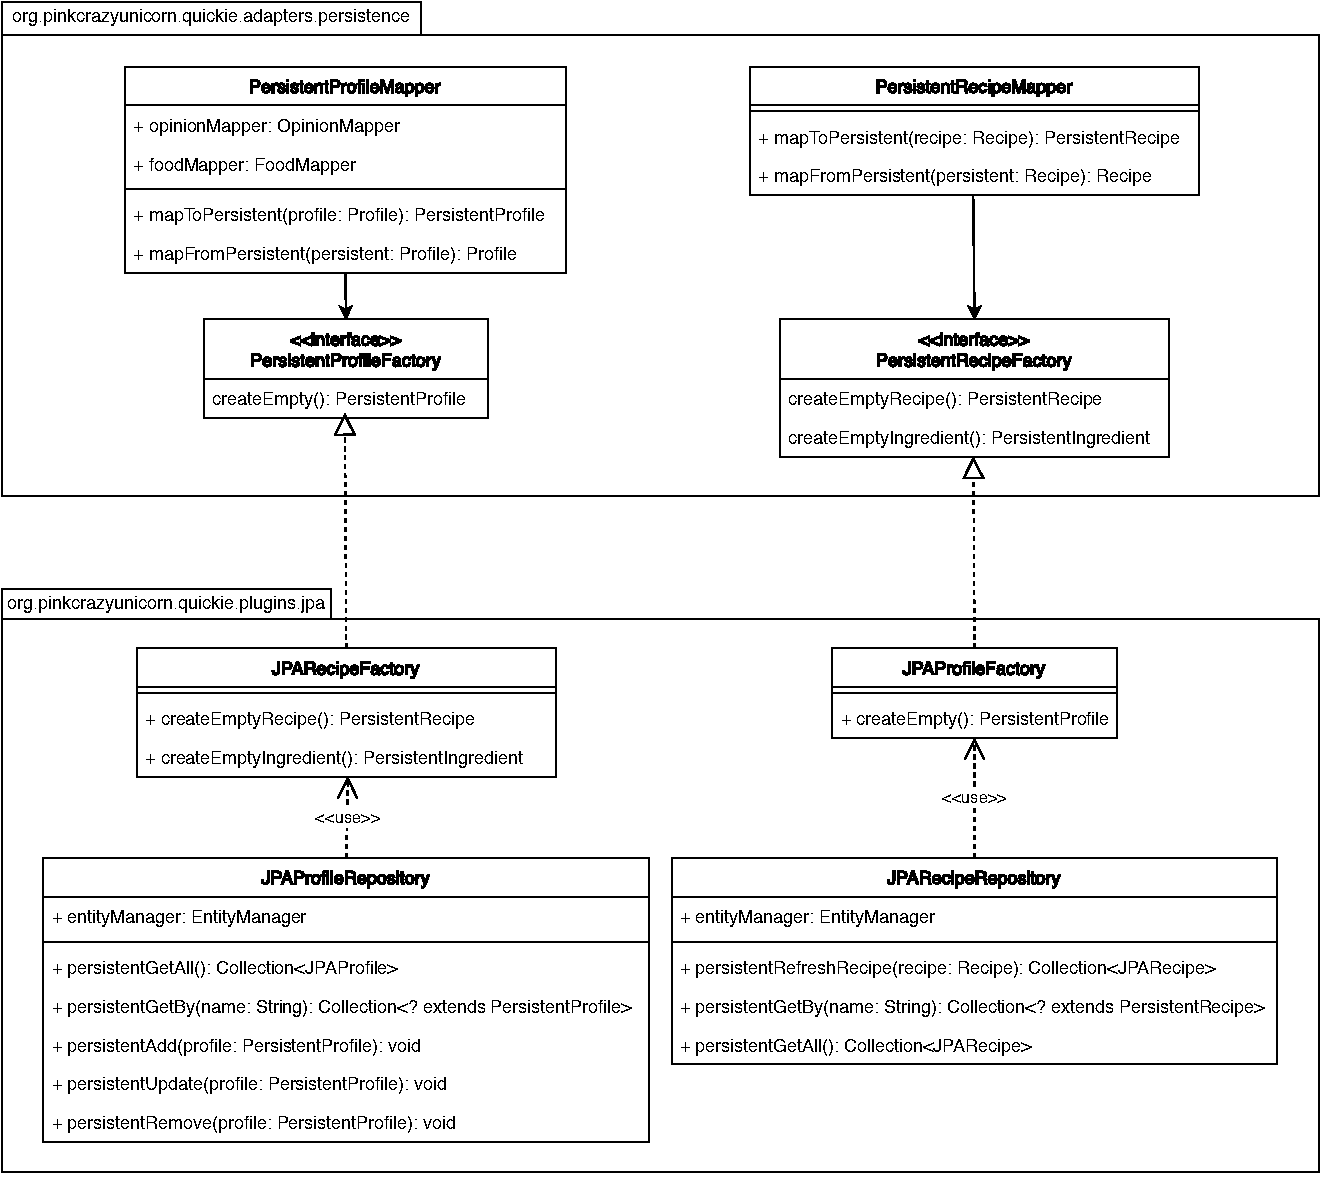
\includegraphics[width=0.98\columnwidth]{../diagrams/factory_uml.pdf}
    \caption{Klassendiagramm der Domäne}
    \label{fig:class-diag-factory}
\end{figure}
